\section{Design}
\label{sec:design}

% Around 5 pages about functional aspects of the FeedApp application.
The main purpose of the FeedApp is to deliver a modern web application that offers a seamless and intuitive experience, allowing users to log in, craft their own surveys and cast votes on existing polls.

\subsection{Use cases}
 \textbf{User Authentication and Authorization}:
In FeedApp, user authentication and authorization are handled using OAuth 2.0 to make logging in secure and easy. When users want to log in, they can either use their FeedApp credentials or sign in through a trusted service like Google. If they choose a third-party login, they are redirected to that provider to confirm their identity. Once they’re logged in, the system gives them a token that lets them interact with the app without having to log in again for every action. This keeps things secure and makes the whole experience smoother for the user.
\medskip

\noindent
 \textbf{Survey Creation}:
One of the main features of FeedApp is letting users create surveys. After logging in, users can go to the "Create Survey" page to start building their survey. First, they give the survey a title. Then they can add multiple polls to it, setting the order of each poll so that everything flows the way they want. Inside each poll, they can add as many options as needed for participants to choose from. Once the user is done creating their survey, it gets saved in the system and is ready for others to participate in. This makes it simple to create detailed surveys with multiple questions and options.
\medskip

\noindent
 \textbf{Voting on polls}:
Voting is another important part of FeedApp. Logged-in users can find active surveys, go through the polls, and select the options they want to vote for. Once they’ve made their choices, they submit their votes, and the system processes them. After the vote is recorded, the results are updated in real time so everyone can see the latest vote counts. This real-time feature makes the app more interactive and lets participants stay up-to-date on how the survey is doing.
\medskip

\noindent
 \textbf{View Survey Results}:
FeedApp also makes it easy to view survey results, both for the person who created the survey and for the people who participated in it. After a survey is published, users can look at the results for each poll. The app shows things like the total number of votes and how the votes are spread across the different options. These results update automatically whenever new votes are added, so the data is always current. This feature helps creators see how their surveys are performing and gives participants a clear view of the outcome.

\begin{figure}[thb]
	\centering
	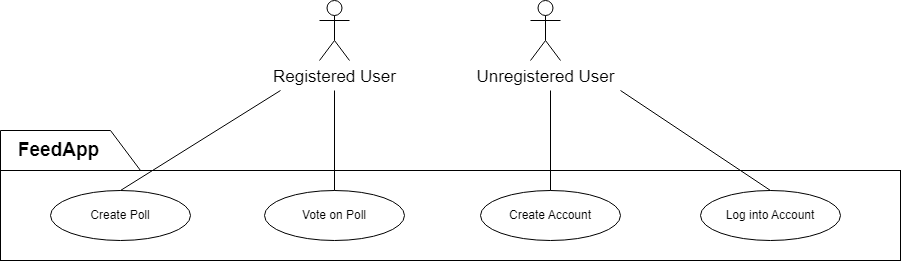
\includegraphics[scale=0.5]{figs/usecase.png}
	\caption{Use Case}
	\label{fig:usecase}
\end{figure}

\subsection{Domain model}
\begin{figure}[!htbp]
	\centering
	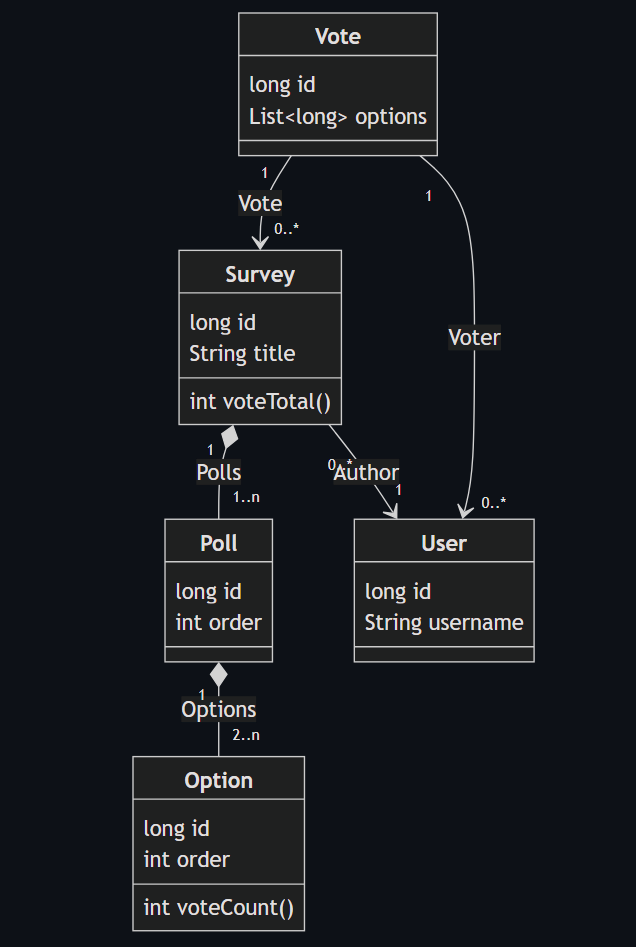
\includegraphics[scale=0.5]{figs/domainmodel.png}
	\caption{The Domain Model.}
	\label{fig:domainmodel}
\end{figure}
The domain model for the FeedApp application captures the core entities and their relationships, providing the foundation for managing surveys, polls, and user interactions. This model ensures a structured and scalable approach to data representation, supporting the application's primary functions such as survey creation, voting, and user management.
\medskip

\subsubsection*{Entities in the Domain Model}

The following entitites can be seen in figure~\ref{fig:domainmodel}:
\smallskip

\noindent
 \textbf{User}:
A User represents an individual interacting with the system, either as a participant in surveys or as an author creating new polls. The Survey entity acts as the central object, representing a collection of polls authored by a user. Each survey is comprised of one or more Polls, which in turn consist of multiple Options that users can select from when casting their votes. The Vote entity captures the act of participation, linking users with the options they select in a given poll.
\medskip

\noindent
 \textbf{Survey}:
A Survey is the primary container entity, representing a collection of polls authored by a user. Each survey has a unique id and a title describing its purpose. The voteTotal() method calculates the total number of votes across all associated polls, providing a quick summary of survey engagement.
\medskip

\noindent
 \textbf{Poll}:
The Poll entity is a component of a survey, representing a single voting instance within it. Polls are ordered using the order attribute, ensuring that their sequence within a survey can be maintained. Each poll is linked to multiple options, allowing users to select from predefined choices.
\medskip

\noindent
 \textbf{Option}:
Options are individual choices within a poll. Each option is uniquely identified by an id and has an associated order attribute to define its position within the poll. The voteCount() method calculates the number of votes an option has received, enabling detailed poll result analysis.
\medskip

\noindent
 \textbf{Vote}:
The Vote entity captures user participation in polls. A vote links a user to specific survey options they have chosen, ensuring accurate representation of voting behavior. The entity includes a unique id and relationships with the User, Survey, and Option entities.
\medskip

\noindent
\subsubsection*{Relationships}
\noindent
The relationships between these entities are key to the domain model's functionality. A survey can have many polls, and each poll must have at least two options to be valid. Votes are associated with both users and surveys, reflecting the choices made by participants. This model not only reflects the application's functional requirements but also ensures data integrity through these defined relationships. Additionally, the use of attributes such as timestamps and unique identifiers allows for detailed analytics and user tracking, which are essential for the platform's growth and adaptability.
\medskip

\noindent
This domain model provides a solid foundation for implementing the core features of FeedApp, including survey creation, user participation, and vote aggregation. Its design ensures that the application can scale to accommodate a growing number of users and complex interactions, while maintaining a clear and manageable structure.

\subsection{Architecture}
\begin{figure}[!htbp]
	\centering
	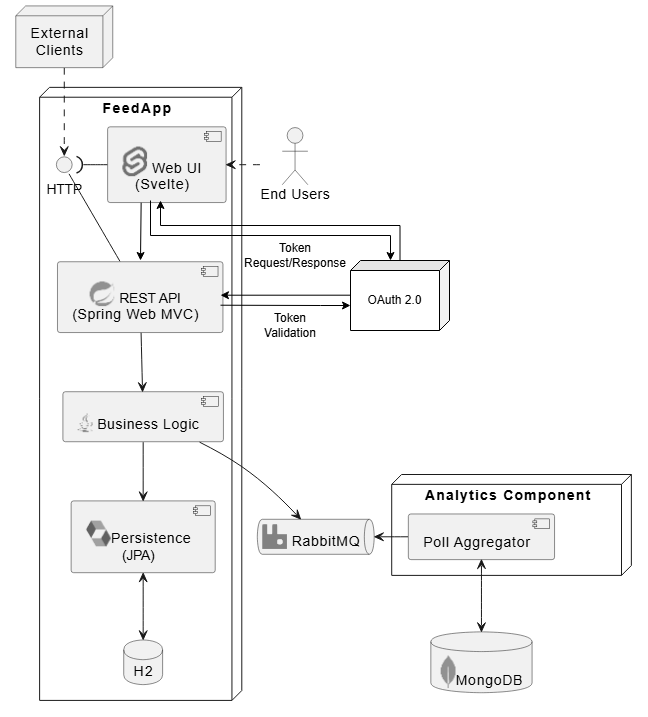
\includegraphics[scale=0.5]{figs/architecture.png}
	\caption{Architecture}
	\label{fig:architecture}
\end{figure}

\medskip

\noindent
The architecture of the FeedApp as shown in figure~\ref{fig:architecture}  is a layered, modular design that leverages modern frameworks and tools to ensure scalability, security, and maintainability. It comprises three primary layers: the frontend, the backend, and the supporting infrastructure. This design follows the principles of separation of concerns, ensuring that each layer is independent and focused on its specific role, yet works seamlessly with others.
\medskip

\noindent
The frontend is implemented using Svelte, a reactive framework that enables the creation of a lightweight Single Page Application (SPA). This layer serves as the primary interface for users, providing an interactive and responsive experience for creating and participating in surveys. The SPA communicates with the backend through HTTP requests, incorporating token-based authentication via OAuth 2.0 to ensure secure interactions.
\medskip

\noindent
The backend is constructed using Spring Boot, with a RESTful API developed through Spring Web MVC. This API acts as the mediator between the frontend and the business logic layer, handling requests from the Web UI and ensuring secure and efficient processing of user data. The business logic layer implements the core functionalities of the application, such as survey and vote management, and interacts with the persistence layer to retrieve or store data.
\medskip

\noindent
The persistence layer employs a hybrid database approach, utilizing PostgreSQL for structured data and MongoDB for unstructured or semi-structured data. The relational database is used for managing users, surveys, polls, and votes, ensuring consistency and reliability. Meanwhile, the non-relational database supports the analytics component by storing aggregated data and logs for flexible querying and reporting.
\medskip

\noindent
To facilitate communication between components and enable scalability, the architecture incorporates RabbitMQ as a message broker. This ensures asynchronous processing of tasks such as vote aggregation and analytics updates, allowing the system to handle high loads without compromising performance. The analytics component processes messages from RabbitMQ and stores the results in MongoDB, enabling real-time insights and historical analysis.
\medskip

\noindent
Security is a key focus of the architecture. Authentication and authorization are implemented using OAuth 2.0, which ensures that only authenticated users can interact with the system. Tokens issued by an external or custom Authorization Server are included in API requests to verify user identity and enforce access control.
\medskip

\noindent
The layered architecture of FeedApp ensures that it is both modular and extensible. Each component operates independently, making the system easier to test, maintain, and scale. The use of modern technologies and best practices guarantees a robust platform capable of supporting a wide range of user interactions, from survey creation to advanced analytics. This architectural design not only meets the current requirements but also provides a strong foundation for future enhancements and growth.





%You may have a look at the \href{https://github.com/selabhvl/dat250public/blob/master/projectdescription/README.md}{Examples on GitHub}.

